\chapter{Nuclear Models}

Where is the peak for elastic ep scattering? e.g. what beam energy maximizes ep elastic event count rate?

Please describe again exactly what is and what is the cause of gluon saturation?
$Why does gluon saturation scale as A^(1/3)?$

BE2 vs E2  There are no stable nuclei with mass numbers five or eight.  

    \section{Weak and Strong Isospin}
        \indent Before the quark model, the proton and neutron were just thought of as two states of one particle, the nucleon. Protons were isospin +1/2 and neutrons were isospin -1/2. After the quark model, this got renamed to strong isospin - assigned to up and down quarks - up is isospin 1/2, $I_3 = +1/2$, down is isospin 1/2, $I_3 = -1/2$. Quarks also have strangeneess charmeness topness and bottomness, which follow from the above. \\
        \indent Weak isospin, T, decides how a particle behaves in weak interactions, and belongs in the SU(2) group. Charged leptons and down-type quarks have $T_3 = -1/2$, neutrinos and up-type quarks have $T_3 =  +1/2$. \\
        "Weak hypercharge", Y, belongs to the U(1) group. Due to spontaneous symmetry breaking and the non-zero VeV of the Higgs field, only a special combination of these quantities is conserved, e.g. $Q = T_3 + 1/2 Y_W$\\
        \href{https://www.youtube.com/watch?v=dquBZfagEmQ}{Helpful Video}

\section{Phase Shifts}
    From Joe: I've read through Wong 3-7 and appendix B.  These were pretty useful for getting an idea of phase shift measurements.  Phase shift measurements are one way to study an interaction potential.

%and is it right to say NN int models interactions between 2 nucleons, while fermi/liquid drop / shell is an effective model for many nucleons because we can't calculate NN-int across n! pairs of n %nucleons in a nucleus

%fermi gas --> momentum distributions of nucleons?
%It might also be why we can use single particle wave functions to describe nuclei
%so maybe it's also fermi gas --> Hartree-Fock?
%These are just my initial guesses.  I'll let you know if I find a real answer
%I know Or's pretty big into why the momentum distributions don't match the Fermi distribution
%Yeah, I think the whole thing with SRC's is they can have momentum way above the fermi momentum

If you have a central potential, the wave function describing the interaction of two particles can be split into a radial and angular part.  Then, you can look at just the radial part as the potential goes to zero.  Non-zero potentials only change the radial part of the equation through phase-shifts.



Using partial wave analysis, it is possible to write the total elastic-scattering cross-section as a function of the phase shifts, which are functions of energy.



Liquid drop model – nuclear forces on nucleus on surface is different than on intereior  gives you shape deformations



Then, cross-section measurements can be used to probe the nature of the interactions.



I'd recommend a quick read through of Wong 3-7 at least.  If you have time, I thought appendix B was useful too.  Also feel free to just ask me more questions.



Nature of interactions could be things like (iso)spin-dependence or range of the potential.



Energy dependence seems to be the biggest factor.


Nucelar radius goes as R = r0 * ato the 1/3, with r0 = 1.2 fm

  measure $V_r$ with phase shift measurements 

know how to write hamiltonian and HF methods

Review tunneling for alpha particles, calculate tunneling, Geiger natal rule
Weisskopf units

        
    \section{Why don't all elements decay to Iron 56?}
        \textbf{Fe 56 has the highest binding energy per nucleon of all elements, so why don't all elements just decay to about iron 56?}\\
        \newline
        \indent The nucleon has to go through a deformed state first, which has a higher energy than the current nucleon, so unless it can overcome this activation energy, it does not happen: \href{https://www.youtube.com/watch?v=cMYJKjBHIiA}{video explanation}
 
     \begin{figure}[H]
        \centering
        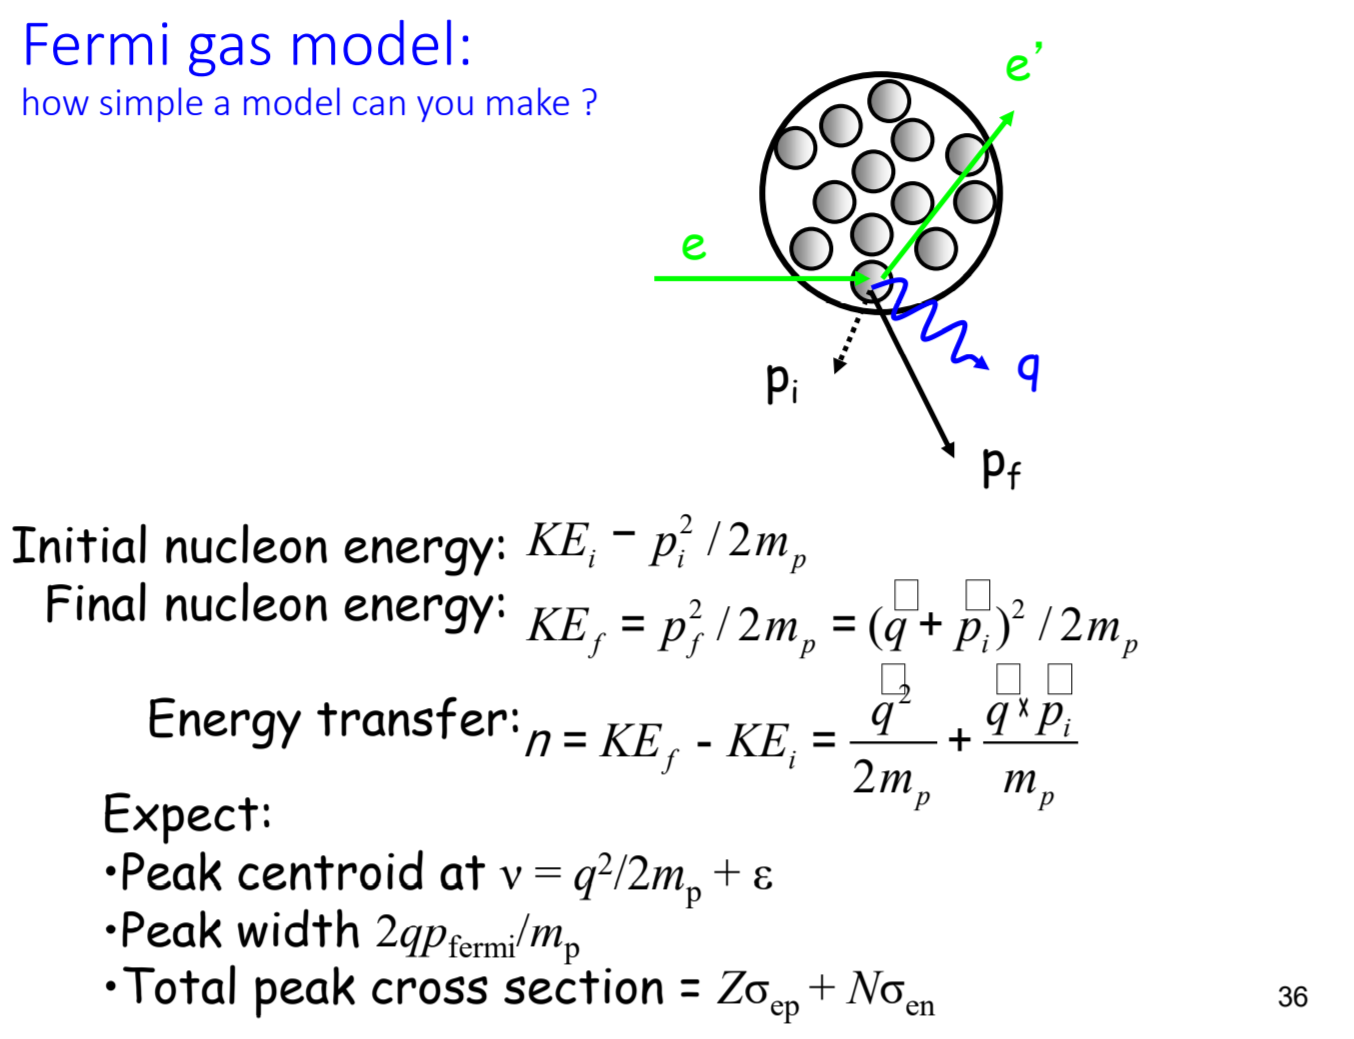
\includegraphics[width=6cm]{NuclearPhysics/modules/nuclear-models/pics/fermi-gas/fg-1.PNG}
        \caption{NN Interaction Potential}
    \end{figure}       
    
    
     
     \begin{figure}[H]
        \centering
        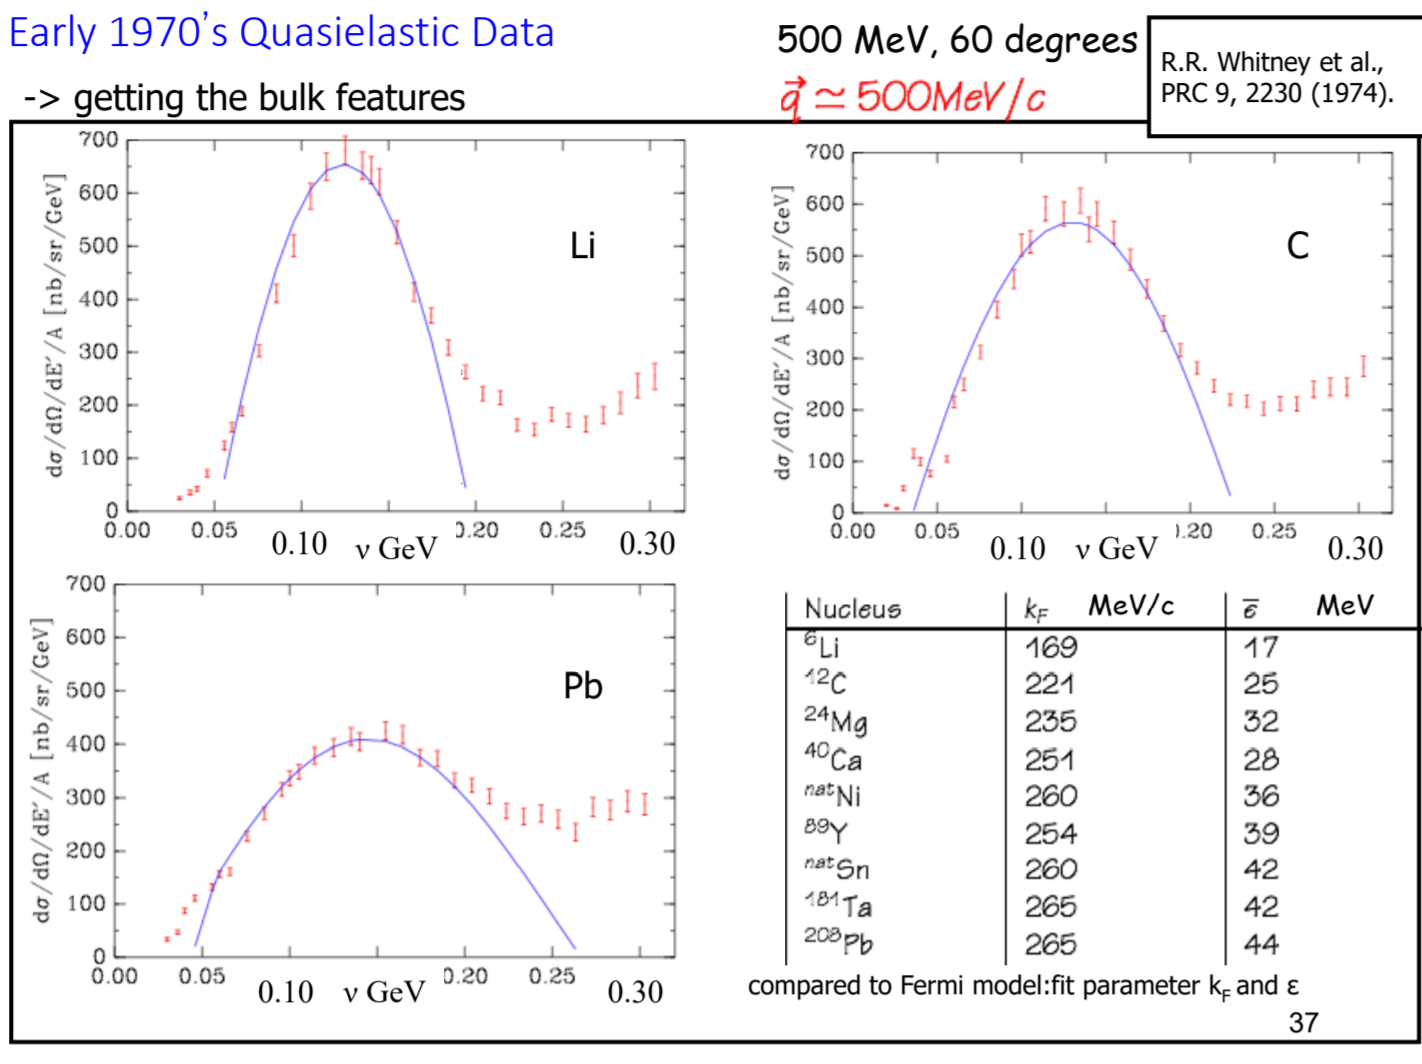
\includegraphics[width=6cm]{NuclearPhysics/modules/nuclear-models/pics/fermi-gas/fg-2.PNG}
        \caption{NN Interaction Potential}
    \end{figure}       


 
     \begin{figure}[H]
        \centering
        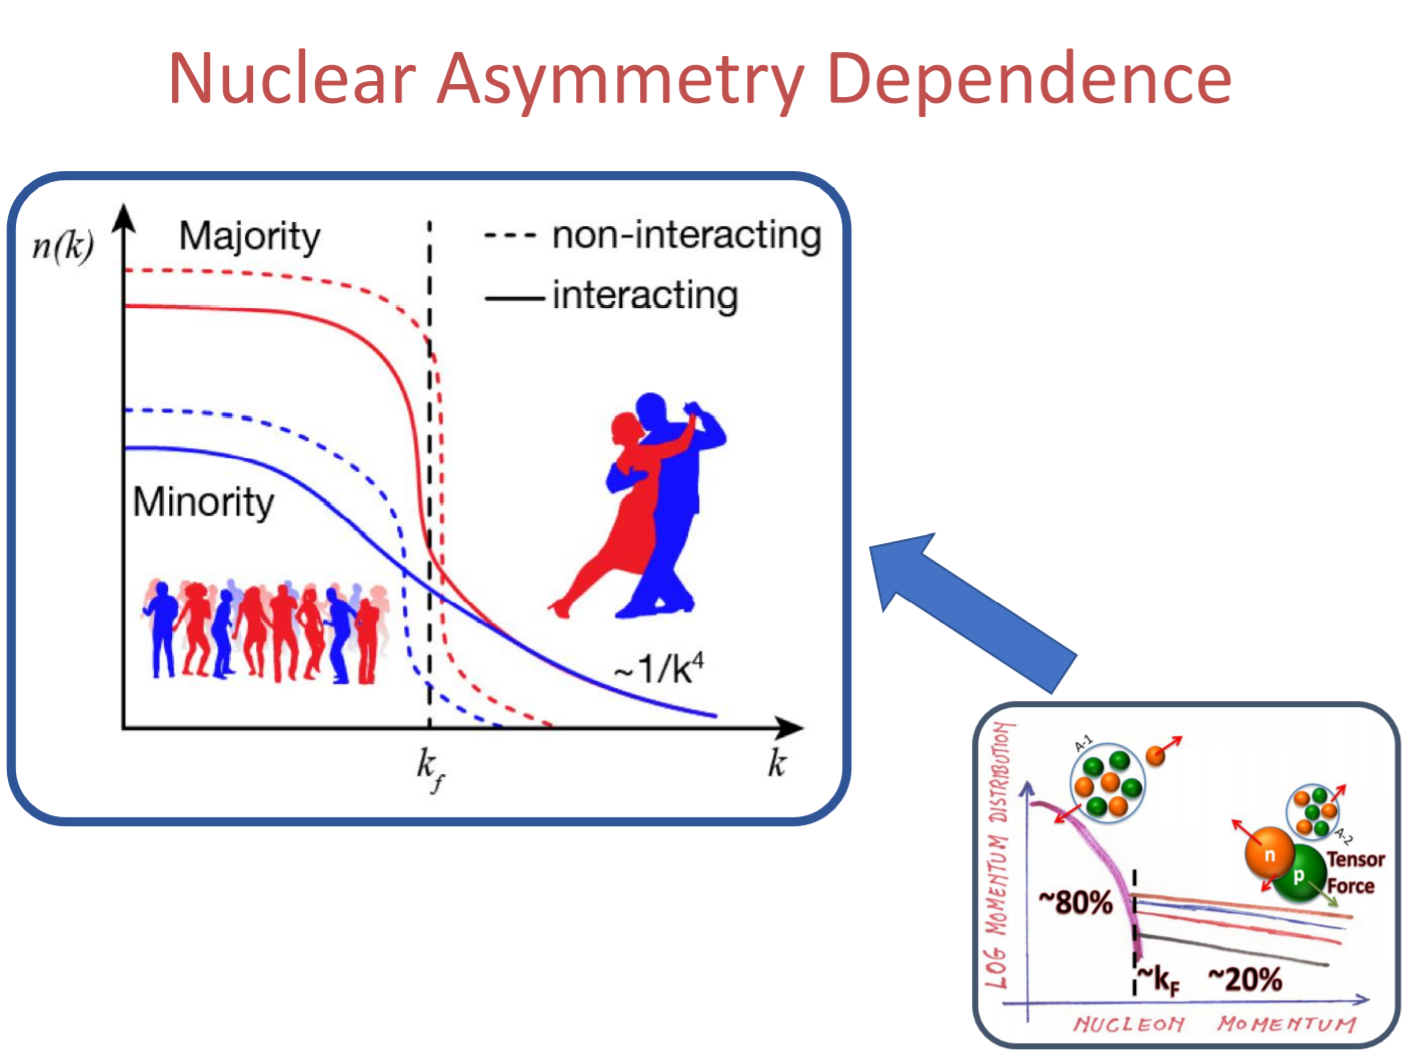
\includegraphics[width=6cm]{NuclearPhysics/modules/nuclear-models/pics/fermi-gas/pairs.PNG}
        \caption{NN Interaction Potential}
    \end{figure}       
    
    
     
     \begin{figure}[H]
        \centering
        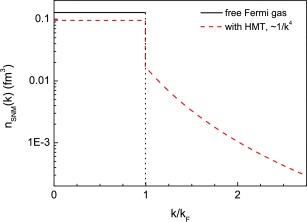
\includegraphics[width=6cm]{NuclearPhysics/modules/nuclear-models/pics/fermi-gas/fermi-mom.png}
        \caption{NN Interaction Potential}
    \end{figure}       

Spectral Functions
Unique Parity states
What is the Yukawoa potential
What is nuclear shadowing and nuclear anti shadowing
Schiff moments
Kurie plot

AV-18!

    \section{Fermi Gas Model}
    Quasielastic provides proof that fermi gas model works - grab slides from Or's notes. 
        \indent Nuclei have a high modmnetum tail - n(k$>k_f$) = a (A/d) *$n_d(k)$ - 20 to 25\% of the nucleons have a high momentum! (meomntumom above the fermi momentum). Maybe the high momentum is coming from nucelon pairs (SRC). how would we probe this? Two nucleon knockout! - break up the pair, detect both nucleons, then reconstruc the inital state. Can cut on kinematics (xB greater than 1, high Q2 (around 2 Gev2), anti-parallel kinematics. Since we have high q2 we can use "Eikonal" approximation for FSI. Correlations are dominated by np pairs - pp only a few percentage of all pairs. - 90\% np, 5\% pp SRC. Also is evidence of tensor force somehow?\\
        SRC dominates momentum distribution for k greater than 300 MeV, account for 25\% of nucleons in nuclei. 18 times more np SRC pairs than pp. Dominant NN forces is the tensor force. \\
        \newline
        \indent Treat the nucleus as a fermi gas constrainted to voluem V. Assume a simple poteintal, solve the schrodinger equation, get quantized momenta. We can get Efermi just from these calculations, and estimate the depth of the nuclear potetnialwell. E fermi is the kinetic energy of the highest occupied orbit int he degenerate gas (smallest binding energy). Since there is no interaciton between particles, it is also equal to the toatl energy (since there is zero potential energy) Because of pauli exlusion, most collisions are prohibited and so non-interacting fermi gas is a reasonable model. 
    \section{Liquid Drop Model}
        \subsection{Weizsacker Semi-Empirical Mass Formula}
            \indent Used to approximate the mass and other properties of a nucleus from its protons and neutrons, assuming the liquid drop model. It does a good job approximating the atomic mass, but fails to explain the existence of magic numbers, which are explained well in the shell model. \\
            
            Provides a good fit for heavier nuclei, but particularly poor fit for very light nuclei, such as helium 4, since it does not account for the shell structure.\\
            
            By maximizing the binding energy with respect to Z, one would fine the best neutron to proton ratio for a given atomic weight, which is roughy 2 for light nuclei, but for heavy nuclei the ratio grows in good agreement with the experiment:\\
            
            $\frac{N}{Z} = 1 + \frac{a_C}{2a_A}A^{2/3}$
            
            Using this, we get the most strongly bound nucleus is cooper, which is closed to the measured values of A = 62 (nickel) and A = 58 iron. \\
            
            \begin{equation}
                m = Zm_p +Nm_n -\frac{E_B}{c^2}
            \end{equation}

            \begin{equation}
                E_B = a_VA-a_SA^{2/3}-a_C\frac{Z(Z-1)}{A^{1/3}}-A_A\frac{(A-2Z)^2}{A}-\delta(N,Z)
            \end{equation}
            \myequations{Binding Energy from Semi-Empirical Mass Formula}
 
            
            \subsubsection{Elucidation of Terms}
            
                \indent Begin by treating the nucleus as a drop of incompressible fluid. The formula has five terms:\\
                
                \indent \indent \textbf{Volume term} - Volume is proportional to A, and this term comes from the strong nuclear force. The number of pairs of particles is A(A-1)/2, but since the strong force has such a short range, only nearest neighbor interactions approximately count, which is roughly proportional to A. A because of short range N-N forces. The total kinetic energy is 3/5A$\epsilon_F$, where \myquantities{Fermi Energy $\epsilon_F$ $\sim$ 28 MeV}. Thus $a_V$ $\sim$ 17 MeV\\
                
                \indent \indent \textbf{Surface term} - accounts for loss of binding at surface. This is a correction to the volume term and is also due to the strong force. The nucleons on the surface have fewer nearest neighbors. Can also be thought of as a surface tension term. Since radius is proportional to $A^{1/3}$, the surface area is proportional to $A^{2/3}$\\
                
                \indent \indent \textbf{Coulomb term} - accounts for EM repulsion of protons. Constant is about 0.7 MeV, comes from calculating out electrostatic Coulomb equation. $A^{1/3}$ is the distance parameter, and Z(Z-1) $\sim$ $Z^2$ = charge of the nucleus. \\
                
                \indent \indent \textbf{Asymmetry term} - Coefficient value of about 23 MeV. Accounts for Pauli exclusion principle (N close to Z preferred). A is in the denominator as this is less significant an effect for larger values of A since energy levels are closer together higher up. Note that A-2Z = N+Z-2Z = N-Z. The reason for this is that if there is an asymmetry, the nucleon species with more particles is stacked higher in energy due to Pauli exclusion. The picture below is illustrative of this:\\
                
                \indent \indent \textbf{Pairing term} - Coefficient value of about 12 MeV, accounts for extra binding when pairs couple to 0 angular momentum states. This is again due to Pauli.\\
            
            Ab-initio nuclear calculations are below percent level in terms of accuracy. 
            
        \begin{figure}[H]
        \centering
        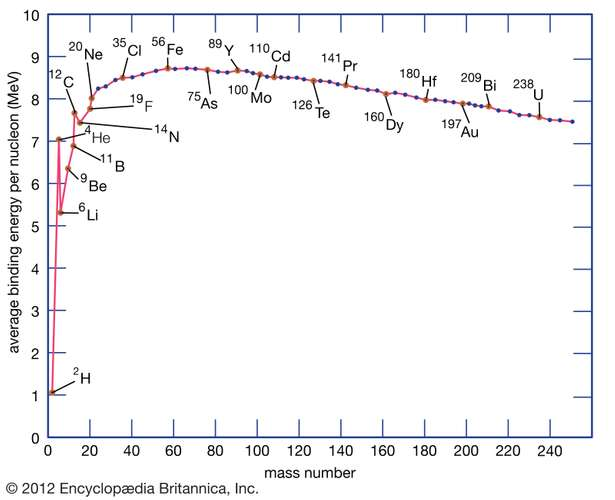
\includegraphics[width=6cm]{NuclearPhysics/modules/nuclear-models/pics/liquid-drop/binding-energy-nucleons.jpg}
        \caption{NN Interaction Potential}
    \end{figure}
            
            \href{https://www.youtube.com/watch?v=oJaq8g8nFZU&t=1s}{Good Video Resource}
    \section{Shell Model}
    
        
Magic numbers(first 5/6)
(2, 8, 20, 26, 50, 82, 126)



J = L + S
$J^2 = L^2 + S^2 + 2LS$
LS = ($J^2 -L^2 -S^2$)/2
LS = ( j(j+1) - l(l+1) - s(s+1))/2
L = 0 --> LS = 0

LS
L2 = m_max2 + m = (mmax (mmax +1))
j = l + 1/2
LS = (l+1/2)(l+3/2) = -l(l+1) - 3/4 = L h2/2

So term Lh2/2 positive term --> pulls energy down

xxx-pics-energy-split
        \indent Consdier the mena field Hamiltonian which neglests residual interactions. Assume a harmonic oscillator potential, get out energy levels. There is l.l and l.s terms . The l.l term is added to diminish the effect of the increasing potetnal at the surface and beyond. It is not good enough to get all the magic numbers. The second term is the spin-orbit interaction and gives all the correct magic numbers up to some high value. 
    
        Question - how come the most dense strongly interacting, many body system in nature can be approximated using a mean field? IN short, Pauli Blocking)
        Bohr-Mottelson collective model
        Notes:
        Double magic nuclei are spherical symmetric
        Adding nucleons or exciting the nuclus breaks the spherical symmetry which creates shape deformation
        SISIS
        What is the weak charge of the proton? (0.08) Of the neutron? (-1)
        
        Most cases will be quadrupole deformed with axial relection symmetry - either prolate (football) or oblate (disc)
        
        Exotic nuclei have more complex deformation (e.g. octopole) with vast implications for BSM searches in atomic EDMs - example - study of pear shaped nuclei - any measurable electric dipole moment should be amplified in such nuclei. Measuring electric octupole transition strengths in for example 220Rn or 224 Ra. $^{224}\!\text{Ra}$
        
        \textbf{Question} How can octupole deformation in nuclei relate to time-reversal violation?
        
        Relation between number of form factors and spin

        \begin{figure}[H]
            \centering
            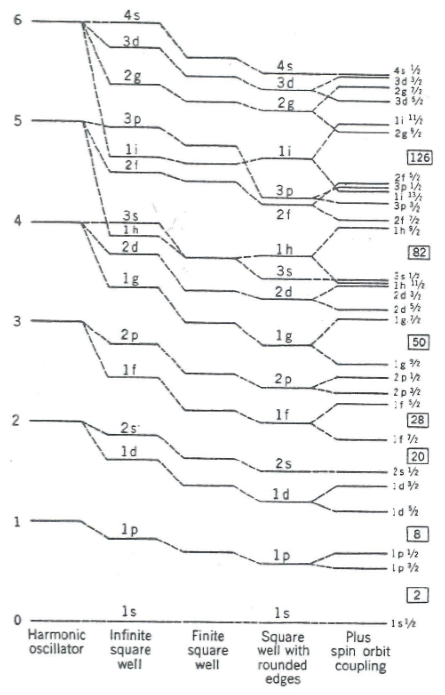
\includegraphics[width=11cm]{NuclearPhysics/modules/nuclear-models/pics/shell_model/shell_model.PNG}
        \caption{NN Interaction Potential}
        \end{figure}
        
        
        \begin{figure}[H]
            \centering
            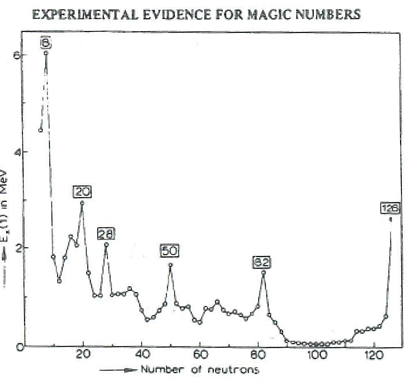
\includegraphics[width=11cm]{NuclearPhysics/modules/nuclear-models/pics/shell_model/E2_energies.PNG}
        \caption{NN Interaction Potential}
        \end{figure}
        
        \begin{figure}[H]
            \centering
            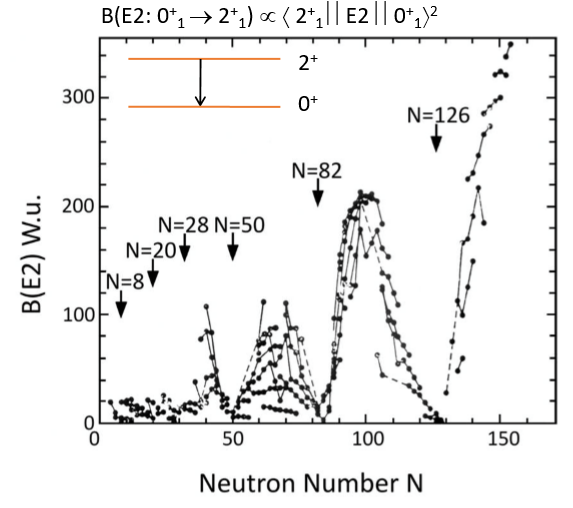
\includegraphics[width=11cm]{NuclearPhysics/modules/nuclear-models/pics/shell_model/BE2_transition_probs.PNG}
        \caption{NN Interaction Potential}
        \end{figure}
        
        
        
         
     \begin{figure}[H]
        \centering
        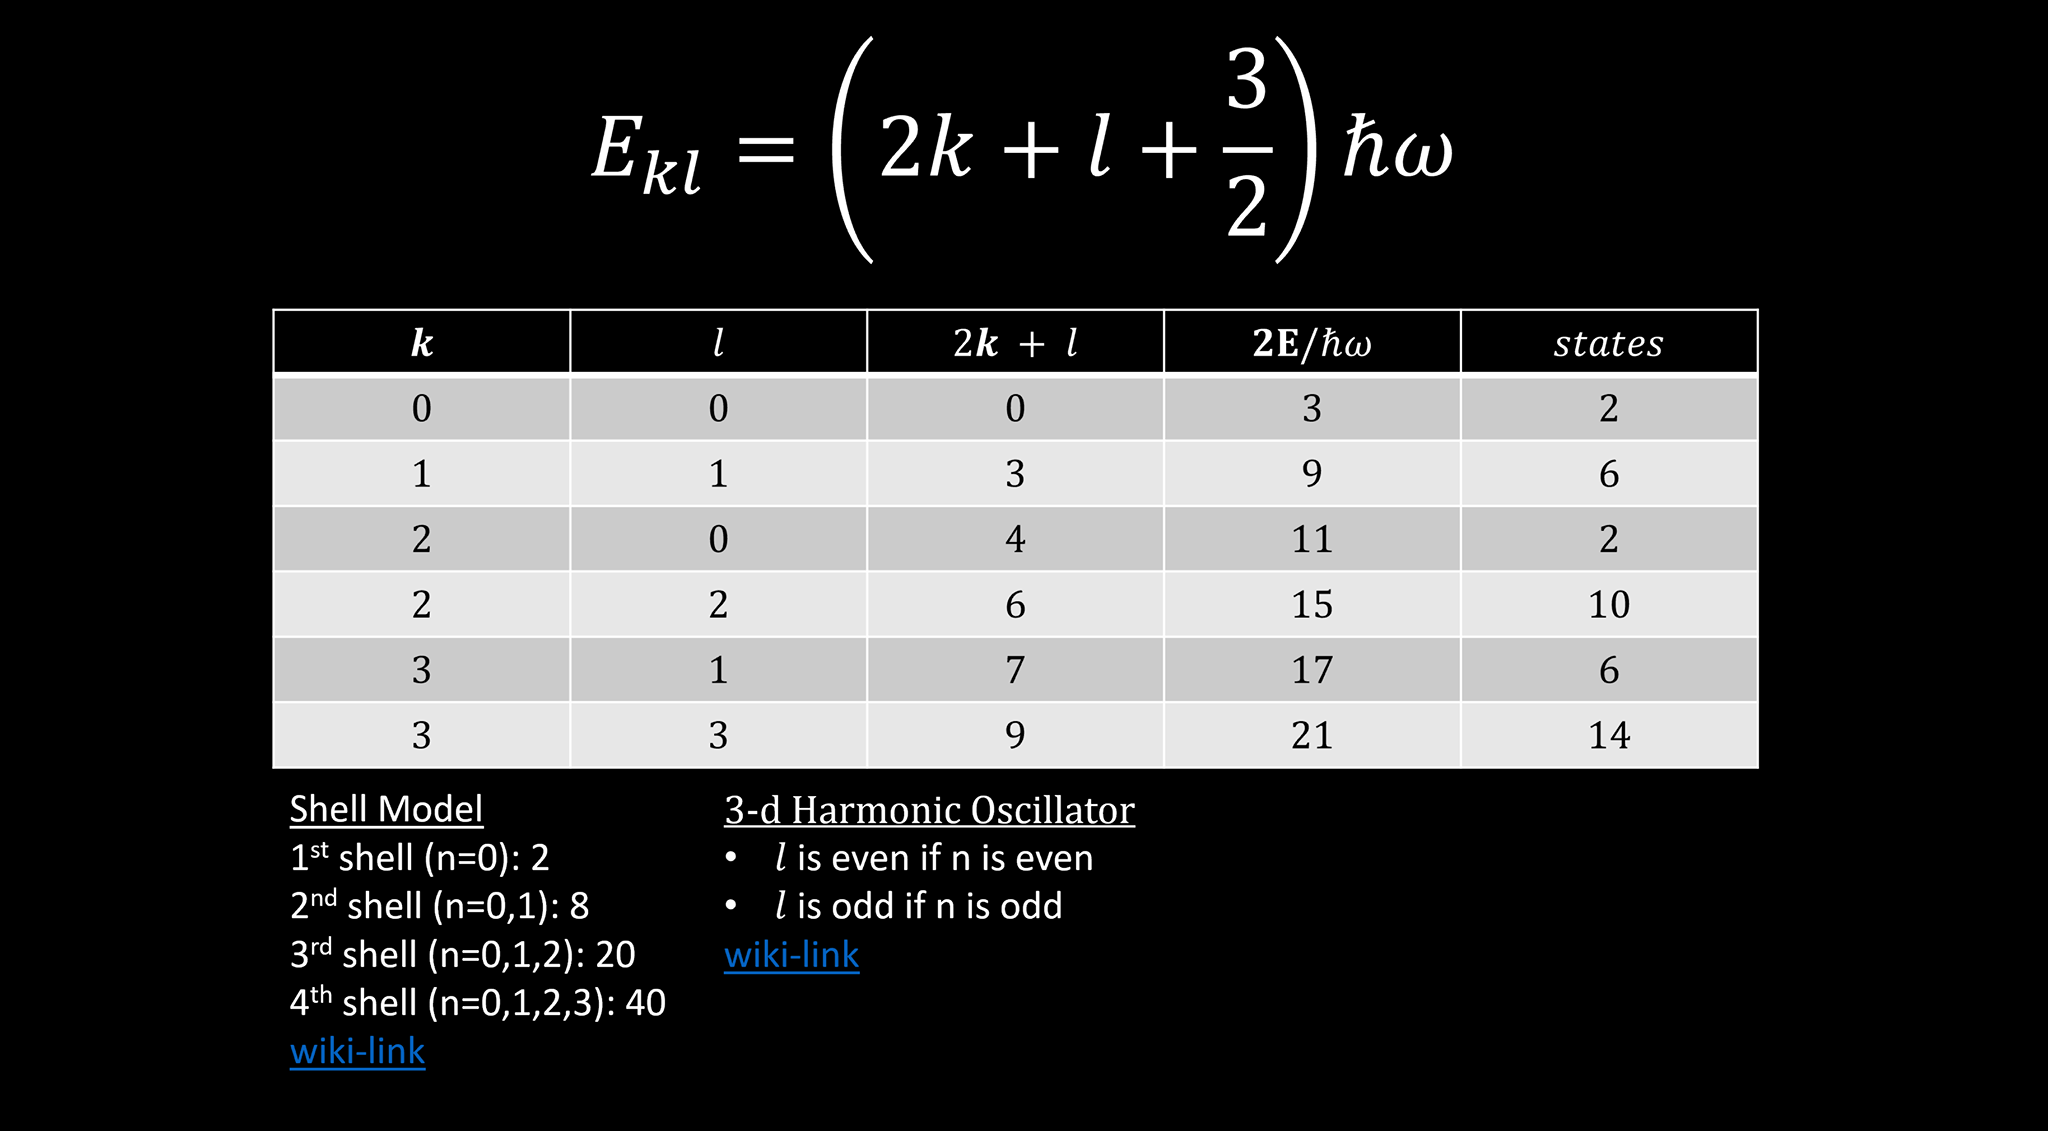
\includegraphics[width=6cm]{NuclearPhysics/modules/nuclear-models/pics/shell_model/shell_model_levels.png}
        \caption{NN Interaction Potential}
    \end{figure}       
    
     
     \begin{figure}[H]
        \centering
        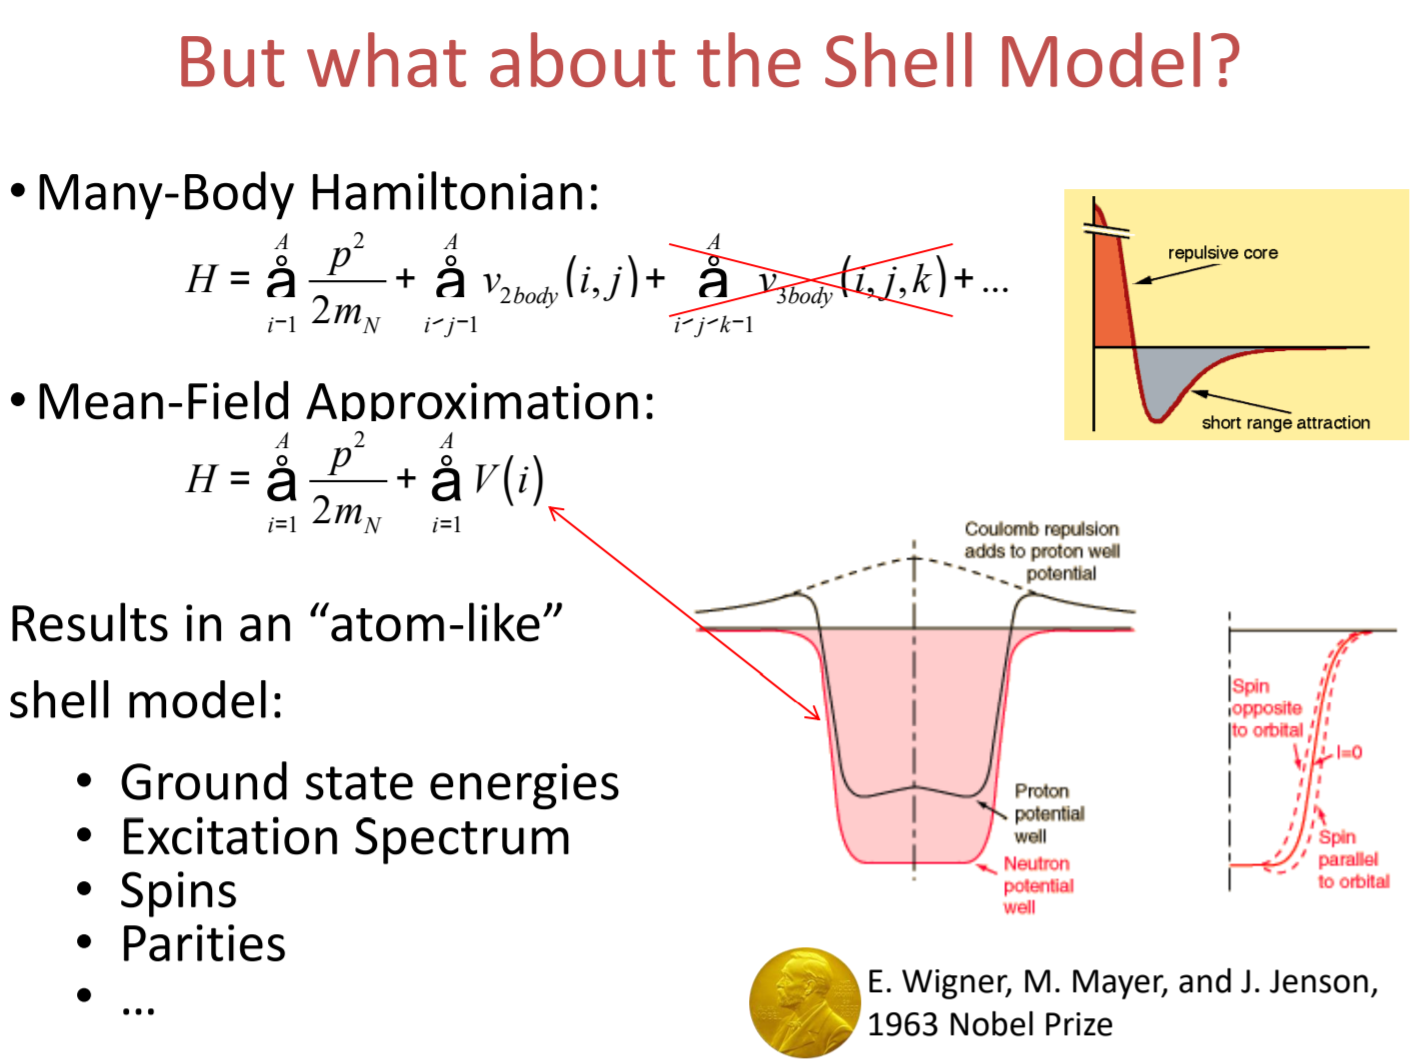
\includegraphics[width=6cm]{NuclearPhysics/modules/nuclear-models/pics/shell_model/shell-model-1.PNG}
        \caption{NN Interaction Potential}
    \end{figure}       
        
        
         
     \begin{figure}[H]
        \centering
        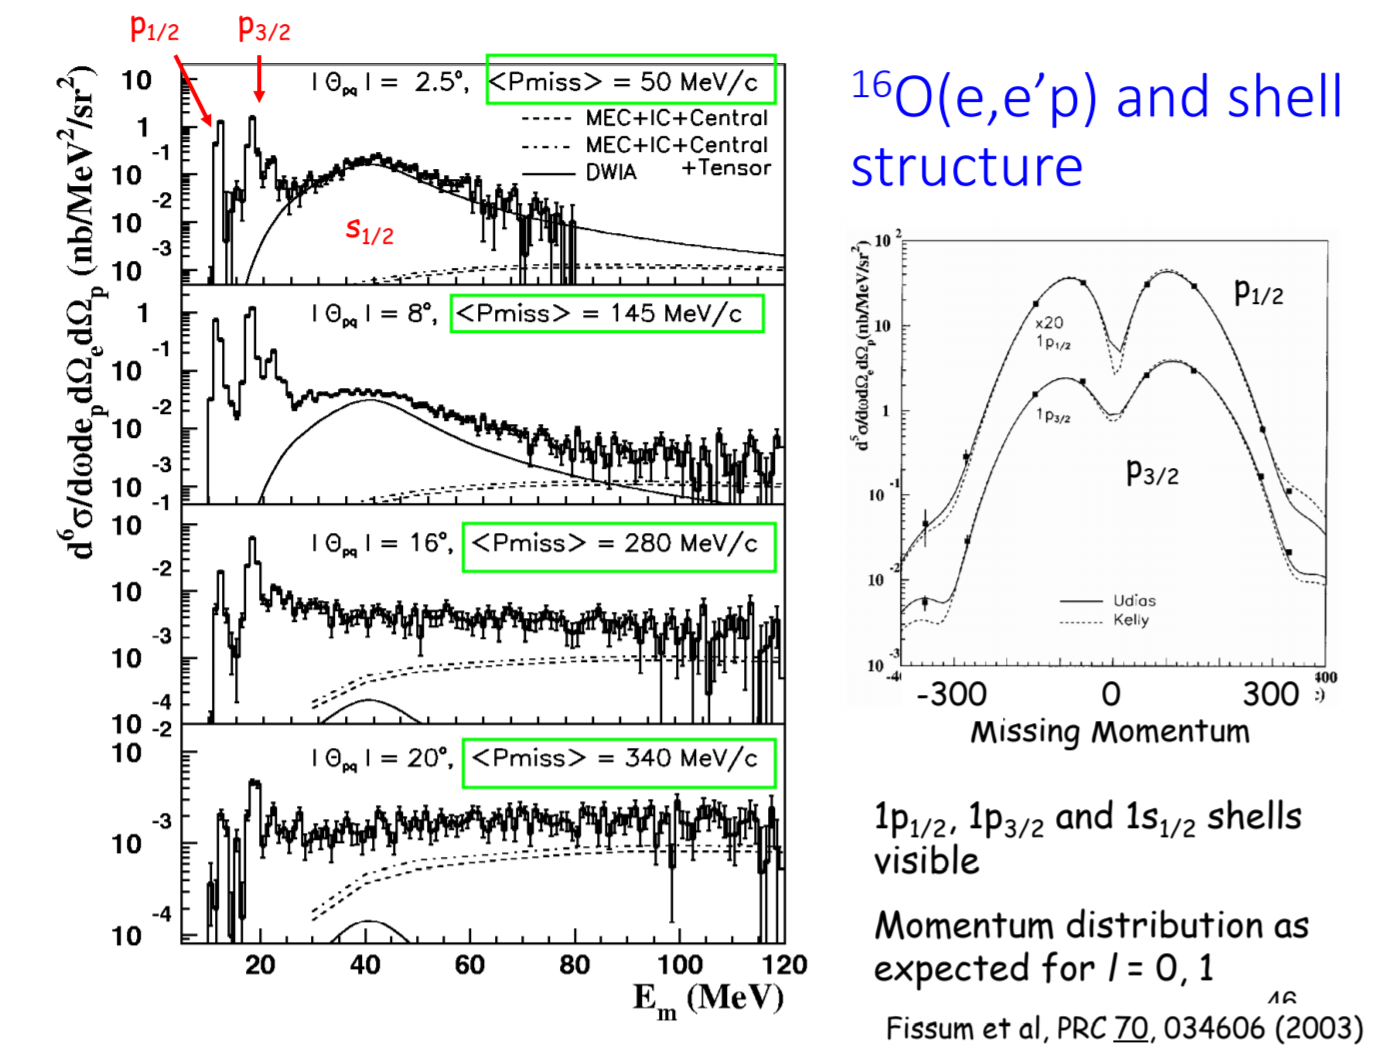
\includegraphics[width=6cm]{NuclearPhysics/modules/nuclear-models/pics/shell_model/shell-model-2.PNG}
        \caption{NN Interaction Potential}
    \end{figure}       
        
        
        
        
    \section{Deformed Nuclei}
        \subsection{Multi pole Expansion}
    \section{Hartree Fock - Woods Saxon and Jacobian thing}
    Outline of method:
    V (Ket Psi)
    Guess a potential (HO, woods saxon, etc)
    Solve for wave function using schrodinger equation
    Based on wavefunction, determine distribution of nucleons
    Calculate what potential that generates
    Iterate until convergence
    hartree fock resources:
    https://www.youtube.com/watch?v=FhlgBzbuIxk&fbclid=
    Need to know equations
    $https://en.wikipedia.org/wiki/Hartree\%E2\%80\%93Fock_method$
    Born Oppenheimer approximation: assume that the motion of nuclei and electrons can be trated separately - this is justified in that the nuclei are much heavier than electrons, so move much slower, so have almost no kinetic energy and are essentially fixed point charges. 
    \section{Optical model}
\chapter{NN Interaction etc.}


(2) The two nucleons being aligned in spin gives some extra binding. This is a property of the nuclear force, in which there is a term
$S12(r^,r^)=(σ1⋅r^)(σ2⋅r^)−3(σ1⋅σ2)S12(r^,r^)=(σ1⋅r^)(σ2⋅r^)−3(σ1⋅σ2$).
The two nucleons in a zero orbital angular momentum state (state of lowest energy) can only align in spin if they are anti-aligned in isospin, by Pauli exclusion.
The second point is the most important one: nucleons antialigned in isospin can be aligned in spin in an orbital angular-momentum zero state (S-state), by Pauli. 



ji and jaffe sum rules
Tensor force from pion exchange, NN centrality
Review phase shifts (WONG ~ 200)
Look up AV18 potential, other parameters, BONN, Argon potential, etc. 
    Basic observations:\\
    Nuclei are small $\longrightarrow$ zero force at long distances\\
    Nuclei are bound $\longrightarrow$ Must be attractive at intermediate distances\\
    Nuclei don't collapse $\longrightarrow$ must be repulsive at short distances\\
    
    Baryons are the constituents, mesons are the force carriers $\xrightarrow{}$ meson mass defines the range.\\
    Example:
    \begin{equation}
        \text{Pion mass = } 140 \frac{\text{MeV}}{c^2},\quad \hbar c = 200 \text{ MeV fm}, \longrightarrow \frac{200 MeV fm}{140 MeV / c^2} = 1.4 \text{ fm $c^2$}
    \end{equation}
    \myequations{Pion NN Int. Range Estimation}
    
    magic numbers: 2 8 20 50 82 126
    
    \begin{figure}[H]
        \centering
        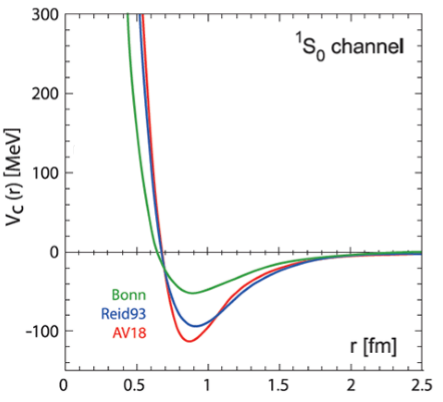
\includegraphics[width=6cm]{NuclearPhysics/modules/nuclear-models/pics/nn-int/nn_potential.PNG}
        \caption{NN Interaction Potential}
    \end{figure}
    
    To build a nuclear model, need to build a hamiltonian, solve a 2 body problem (NN), then solve the many-body problem. This last part is impossible analytically, and means you must resort to \textbf{mean-field / collective approximations}.\\
    
    \myquantities{Nuclear density ~ 0.17 nucleons per $fm^3$}
    

    \section{Properties of Nuclei}
        \subsection{Relative abundances, binding energy, etc. }
    \section{NN Interaction}
        \indent Atomic nuclei are successfully described in terms of hadrons. We start with a NN potential and solve the schrodinger equation. Assumpitons:\\
        1 - potential should depend only on the nucleon separaration, their relative momentum, and their spins\\
        2 - potential should be hermitian\\
        3 - potential should be invariant under rotations\\
        4 - realtive momentum should appear at most lealary (otherwise different poteinail in differet OAM states\\
        5 - limist ourselves to one $\sigma_1$ and/or one $\sigma_2$ because this allows reduction of higher order terms to linear.\\
        \newline
        Through a set of further assumptions we can arrive at isoscalar or isovector interactions. \\
        \newline
        Yukawa theory - the field of nuclear forces corresponds to a particle of mass intermeidate between that of the electron an nucleon (meson) (1935). If we want a foce of about 1 fm, we need a particle of about 200 MeV. 
        
        Phase shifts - way to probe NN interactions?